\documentclass{article}
\usepackage[utf8]{inputenc}
\usepackage{ctex}
\usepackage{amsmath}
\usepackage{indentfirst}
\usepackage{amssymb}%花体字符
\usepackage{graphicx}
\usepackage{geometry}
\usepackage{enumerate}
\usepackage{float} 
\usepackage{subfigure}
\usepackage{fontspec}
\usepackage{pythonhighlight}
\usepackage{listings}
\usepackage[framed,numbered,autolinebreaks,useliterate]{mcode}

\setmonofont{Consolas}
\geometry{a4paper,scale=0.8}
\title{第二次大作业}
\author{计试001 苏悦馨 2204120515}
%\date{}

\begin{document}
\maketitle

\section{P34页大作业}

\subsection{问题描述}
对于两个变量的二次规划问题:$\min f(x) = \frac{1}{2} (x_1^2+\gamma x_2^2), \gamma > 0$。初始值为$x^0=(\gamma,1)$。采用精确直线搜索梯度下降,第$k$次迭代后
\begin{equation*}
    x^k=(\frac{\gamma-1}{\gamma+1})^k
    \left[ \begin{array}{c}
            \gamma \\
            (-1)^k
        \end{array}\right]
\end{equation*}

% 采用归纳法证明,$k=0$时满足$x^0=(\gamma,1)=(\frac{\gamma-1}{\gamma+1})^0 \left[ \begin{array}{c}
%             \gamma \\
%             (-1)^0
%         \end{array}\right]$

% 设$k=N$时满足条件,$k=N+1$时有:
% \begin{equation}
%     \begin{gathered}
%         t^N=\arg\min f(x^N-t\nabla f(x^N))\\
%         \Rightarrow \frac{d}{dt}\left((1-t)^2(x_1^N)^2+\gamma(1-\gamma t)^2(x_2^N)^2\right)=0\\
%         \Rightarrow t^N=\frac{\gamma^2 (x_2^N)^2+(x_1^N)^2}{\gamma^3 (x_2^N)^2+(x_1^N)^2}=\frac{2}{1+\gamma}\\
%     \end{gathered}
% \end{equation}

% \begin{equation}
%     \begin{aligned}
%         \therefore
%         x^{N+1} & =x^N-t^N\nabla f(x^N)          \\
%                 & =(\frac{\gamma-1}{\gamma+1})^0
%         \left[\begin{array}{c}
%                       \gamma \\
%                       (-1)^0
%                   \end{array}\right]
%     \end{aligned}
% \end{equation}

编程证明:
\begin{enumerate}[a)]
    \item $\gamma =1$ 时,一次迭代可以取得最优解;
    \item 对于$\gamma$ 离1不不远的情况,收敛速度很快;
    \item 如果$\gamma \gg 1$ 或 $\gamma \ll 1$时,收敛速度将会非常慢。
\end{enumerate}

\subsection{问题思路}

代码思路:
\begin{enumerate}[a)]
    \item 设置临界误差$\epsilon=1E-10$,计算精确直线搜索梯度下降所需的搜索次数为
    $$
    N=\lceil\frac{\log ((f(x^0)-p\ast)/\epsilon)}{\log(1/c)} \rceil
    $$
    \begin{python}
    ######3-34.py中26-36行
    # 迭代次数N
    e = 1E-10
    if gama[k] == 1:
    N = 1
    else:
    if gama[k] > 1:
    N = math.ceil(
    math.log(0.5*(pow(gama[k], 2)+gama[k])/e)/math.log(gama[k]/(gama[k]-1)))
    else:
    N = math.ceil(
    math.log(0.5*(pow(gama[k], 2)+gama[k])/e)/math.log(1/(1-gama[k])))
    \end{python}

    \item 绘制搜索空间的等高线图,以便直观的看到迭代中$f(x)$的减少量;
    \begin{python}
    ######3-34.py中9-22行
    # 建立步长为0.01,即每隔0.01取一个点
    step = 0.01
    x1 = np.arange(-x1_bound[k], x1_bound[k], step)
    x2 = np.arange(-x2_bound[k], x2_bound[k], step)

    # 将原始数据变成网格数据形式
    X, Y = np.meshgrid(x1, x2)
    Z = 0.5*(X**2+gama[k]*(Y**2))

    # 画出5条线,并将颜色设置为黑色
    ax = plt.subplot(2, 2, k+1)
    contour = plt.contour(X, Y, Z, 5, colors='k', linestyles='dashed')
    # 等高线上标明z(即高度)的值,字体大小是10,颜色分别是黑色和红色
    plt.clabel(contour, fontsize=10, colors='k')
    \end{python}

    \item 由所计算得到的迭代次数$N$,以及问题中给出的$x^k$表达式$ x^k=(\frac{\gamma-1}{\gamma+1})^k\left[ \begin{array}{c}\gamma \\(-1)^k\end{array}\right]$,在已绘制等高线的空间中绘出历次迭代的点$x^k,(k=0,1,\dots,N)$。观察取定$\gamma$时迭代过程中点的分布,即可证明上述结论。
    \begin{python}
     ######3-34.py中37-39行
    x_ = [((gama[k]-1)/(gama[k]+1))**i*gama[k] for i in range(N+1)]
    y_ = [((gama[k]-1)/(gama[k]+1))**i*(-1)**i for i in range(N+1)]
    plt.plot(x_, y_, 'go--', linewidth=1, markersize=3)
    \end{python}
\end{enumerate}

$\gamma$取值:
\begin{itemize}
    \item $\gamma =1$ ;
    \item $\gamma$ 离1不不远的情况,取值$\gamma=0.5,2,5$为例考察;
    \item $\gamma \gg 1$ 或 $\gamma \ll 1$的情况,取值$\gamma=0.01,100$为例进行考察。
\end{itemize}

\subsection{结果与分析}

$\gamma=0.5,1,2,5$的迭代过程如下
\begin{figure}[H]
    \centering
    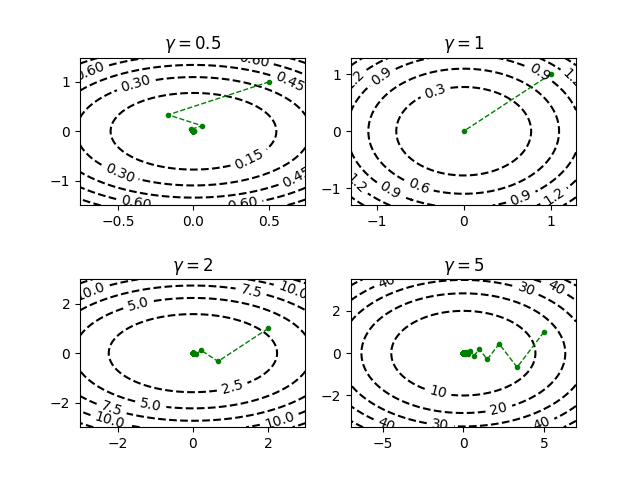
\includegraphics[scale=0.8]{Fig/3-34.png}
    \caption{$\gamma=0.5,1,2,5$的迭代过程}
\end{figure}

$\gamma=0.01,100$的迭代过程如下
\begin{figure}[htbp]
    \centering
    \begin{minipage}[t]{0.48\textwidth}
        \centering
        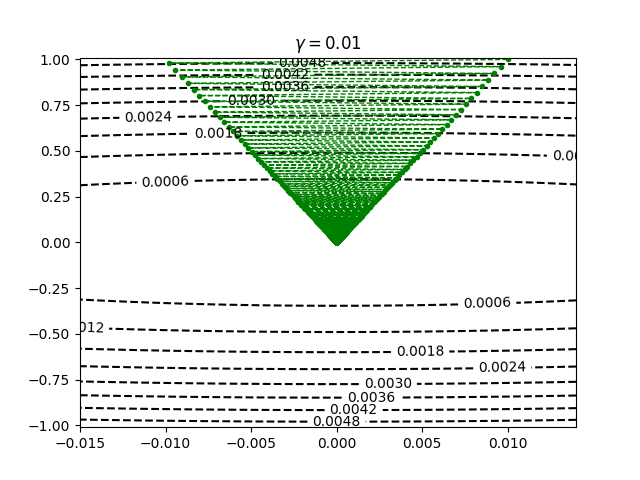
\includegraphics[width=8cm]{Fig/3-34_0.01.png}
        \caption{$\gamma=0.01$}
    \end{minipage}
    \begin{minipage}[t]{0.48\textwidth}
        \centering
        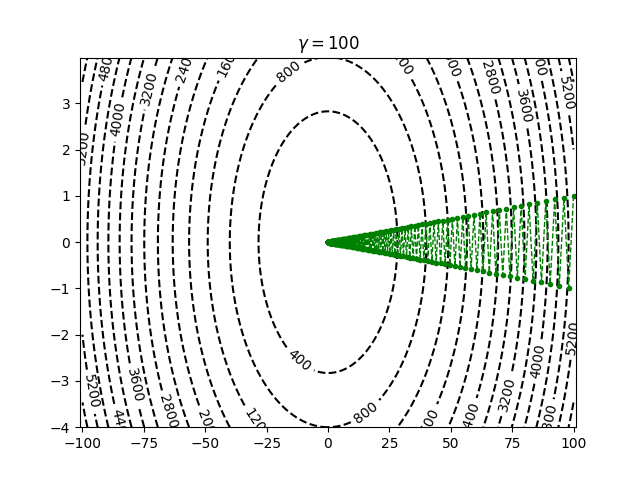
\includegraphics[width=8cm]{Fig/3-34_100.png}
        \caption{$\gamma=100$}
    \end{minipage}
\end{figure}

可以看出,$\gamma =1$ 时,一次迭代可以取得最优解;对于$\gamma$ 离1不不远的情况,收敛速度很快,经过10次以内的迭代便可以收敛到最优解;而如果$\gamma \gg 1$ 或 $\gamma \ll 1$时,迭代路径将通过震荡到达最优解,收敛速度非常慢,从而证明的了要求的结论

\section{P38页大作业}

\subsection{问题描述}
对于$R^2$空间的非二次规划问题$\min f(x)=e^{x_1+3x_2-0.1}+e^{x_1-3x_2-0.1}+e^{-x_1-0.1}$,分析回溯直线搜索采用不同的$\alpha,\beta$值时,误差随迭代次数改变的情况。

\subsection{问题思路}
由梯度下降方法回溯直线搜索算法,下降方向$d^k$满足
\begin{equation*}
    d^k=-\nabla f(x)
\end{equation*}

易求得
\begin{equation*}
    \nabla f(x)=\left(\begin{array}{c}
        e^{x_1+3x_2-0.1}+e^{x_1-3x_2-0.1}-e^{-x_1-0.1} \\
        3e^{x_1+3x_2-0.1}-3e^{x_1-3x_2-0.1}
    \end{array}\right)
\end{equation*}

且易求得,问题的最优解为$\nabla f(x)=0$,解得$\left(x1,x2\right)^T=\left(-\frac{1}{2}\ln 2,0\right)^T$。带入原函数得到问题的最优值为$p^\ast=2.559266697$,从而可画出$f(x^k)-p^\ast$随迭代次数改变的情况。

代码思路:
\begin{enumerate}[a)]
    \item 使用匿名函数设置原函数和其梯度
    \begin{lstlisting}
    %-----Backtracking_line_search.m中3-8行
    %原函数
    f=@(x1,x2) exp(x1+3*x2-0.1)+exp(x1-3*x2-0.1)+exp(-x1-0.1);
    p=f(log(1/sqrt(2)),0);
    %原函数的对x1的偏导
    diff_f_1=@(x1,x2) exp(x1+3*x2-0.1)+exp(x1-3*x2-0.1)-exp(-x1-0.1);
    %原函数的对x2的偏导
    diff_f_2=@(x1,x2) 3*exp(x1+3*x2-0.1)-3*exp(x1-3*x2-0.1);
    \end{lstlisting}

    \item 外循环:判断$\Vert \nabla f(x) \Vert_2<\epsilon$
    \begin{lstlisting}
    %-----Backtracking_line_search.m中23-28行
    nabla_f=[diff_f_1(x(1),x(2)),diff_f_2(x(1),x(2))]';
    norm_f=norm(nabla_f);    
    %进行回溯直线搜索
    while norm_f>e
    \end{lstlisting}

    \item 内循环:通过回溯直线搜索求解$t^k$,使得$f(x^k+t^kd^k)<f(x^k)+\alpha t^k \nabla f(x^k)^T d^k$
    \begin{lstlisting}
    %-----Backtracking_line_search.m中31-34行
    while f(x_(1),x_(2)) > f(x(1),x(2))-alpha(i)*t*norm_f^2
        t=beta(j)*t;
        x_=x-t*nabla_f;
    end
    \end{lstlisting}
    \item 在每次内循环结束后,记录$f(x^k)-p^\ast$,更新$x^{k+1},\nabla f(x^{k+1}) ,\Vert \nabla f(x^{k+1}) \Vert_2$
\end{enumerate}

参数取值:
\begin{itemize}
    \item 初始点$x^0=(0.1,0.1)^T,(4,3)^T,(-89,-5)^T,(20,50)^T$
    \item $\alpha=0.01,0.05,0.1,0.3,0.45,0.49$
    \item $\beta=0.01,0.05,0.1,0.4,0.8,0.95,0.99$
    \item 停止准则$\Vert \nabla f(x^{k}) \Vert_2<10^{-6}$
\end{itemize}


在对于初始点的选择上,选择在初始解附近以及离初始解较远的四个初始点,分别考察回溯直线搜索采用不同的$\alpha,\beta$值时,误差随迭代次数改变的情况,以使结论具有普遍性。

对于确定的初始点$x^0$,遍历$\alpha,\beta $取值的所有组合,来分析回溯直线搜索采用不同的$\alpha,\beta$值时,误差随迭代次数改变的情况。下图中纵坐标为'$f(x^k)-p\ast$',横坐标为迭代次数,纵坐标采用对数坐标。

由于在$\beta$较小时,$\beta$的改变对迭代次数的影响很大,故将不同的$\alpha,\beta$组合的误差随迭代次数变化分为3个子图,迭代次数小于100次,迭代次数大于400次,以及迭代次数在100到400之间,三个区间分别做图。



\subsection{结果与分析}

\begin{figure}[H]
    \centering
    \subfigure{
        \begin{minipage}[t]{1\textwidth}
            \centering
            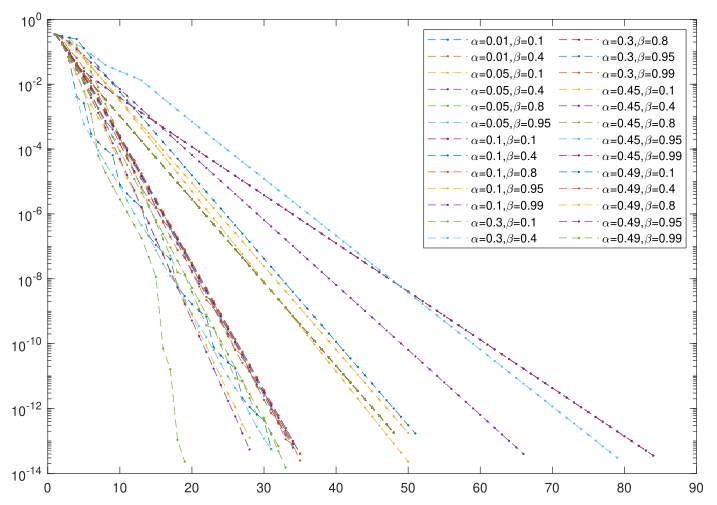
\includegraphics[scale=0.5]{Fig/group1_0101.png}
        \end{minipage}
    }
    \subfigure{
        \begin{minipage}[t]{0.48\textwidth}
            \centering
            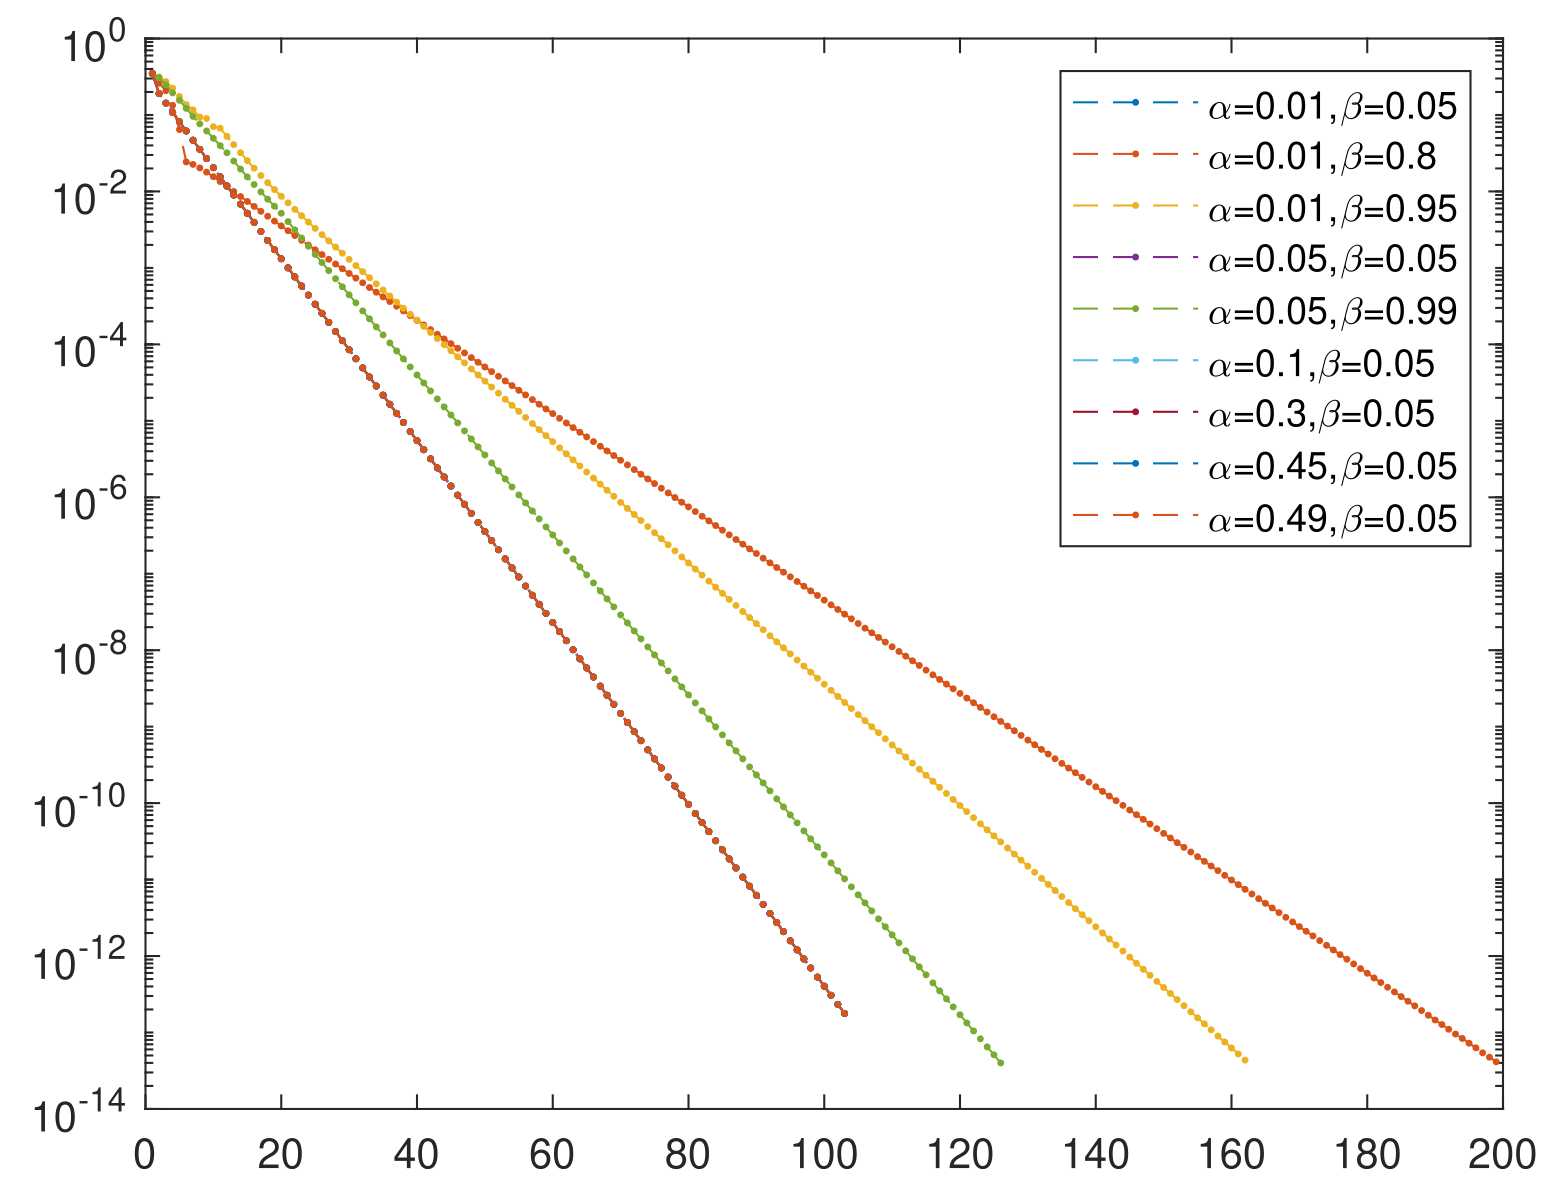
\includegraphics[scale=0.5]{Fig/group2_0101.png}
        \end{minipage}
        \begin{minipage}[t]{0.48\textwidth}
            \centering
            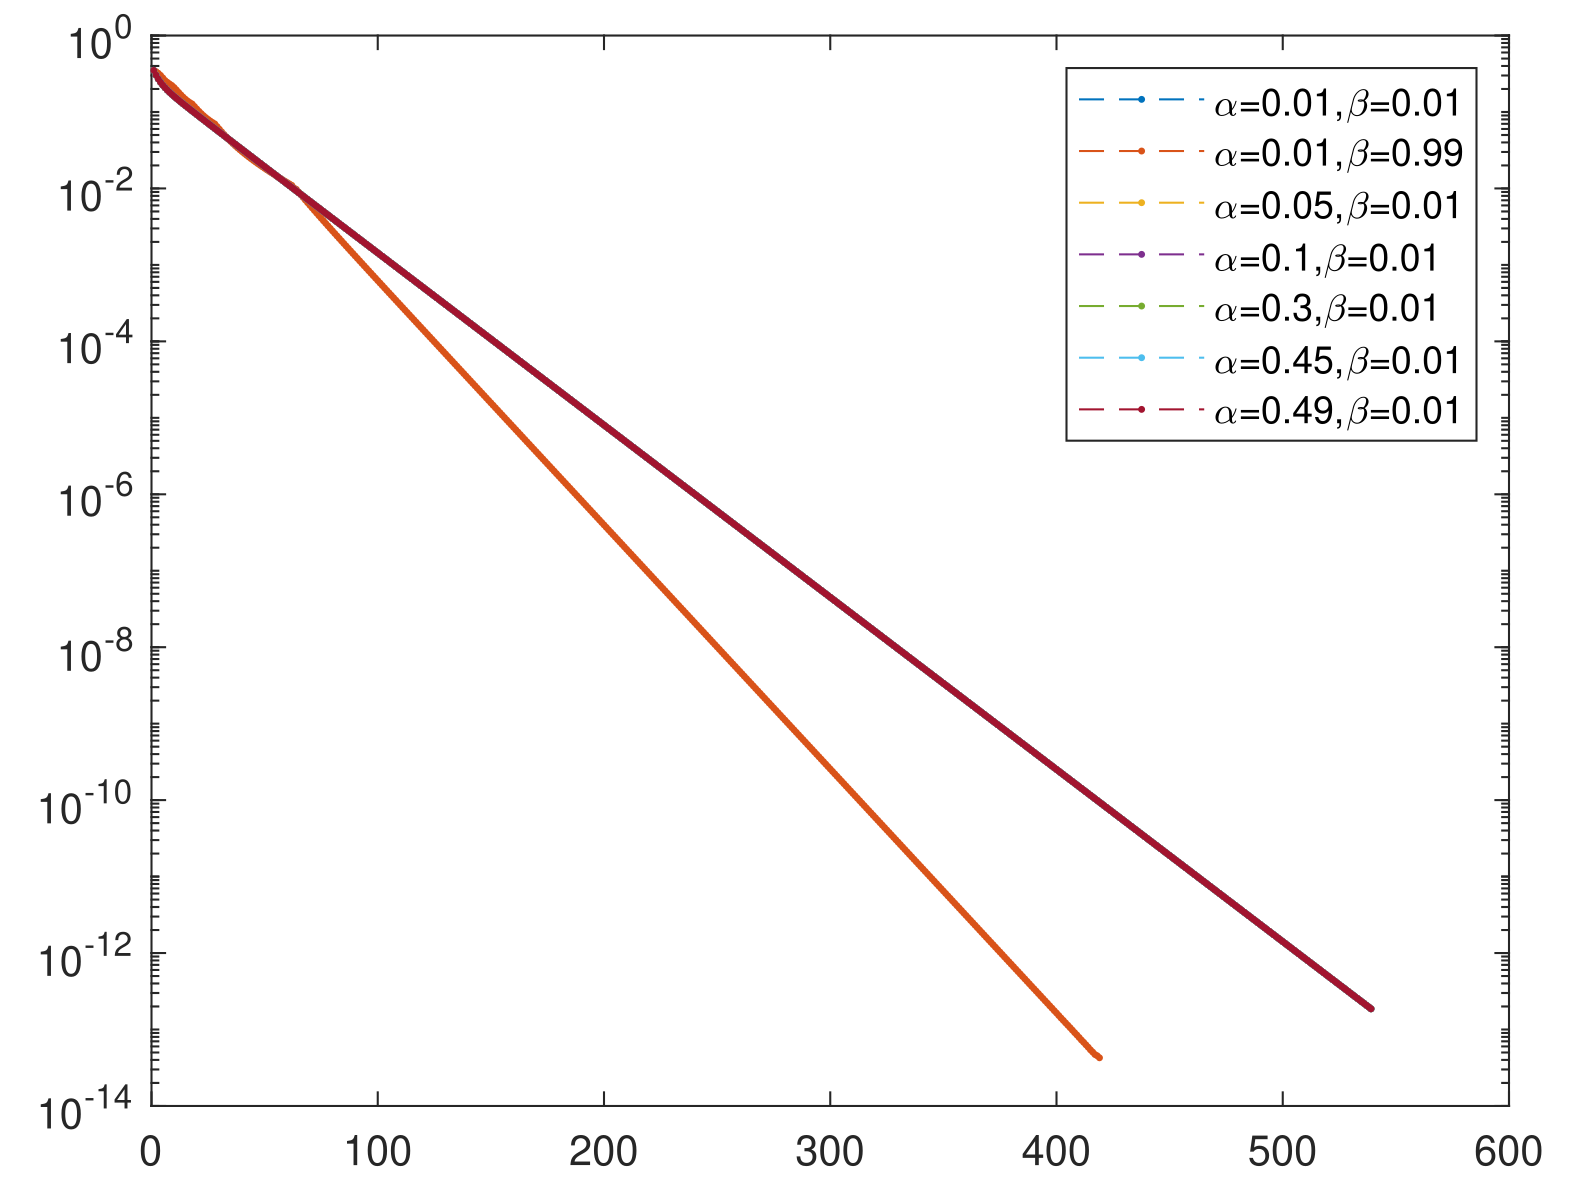
\includegraphics[scale=0.5]{Fig/group3_0101.png}
        \end{minipage}
    }
    \caption{初始点$x_0=(0.1,0.1)^T$}

    \subfigure{
        \begin{minipage}[t]{1\textwidth}
            \centering
            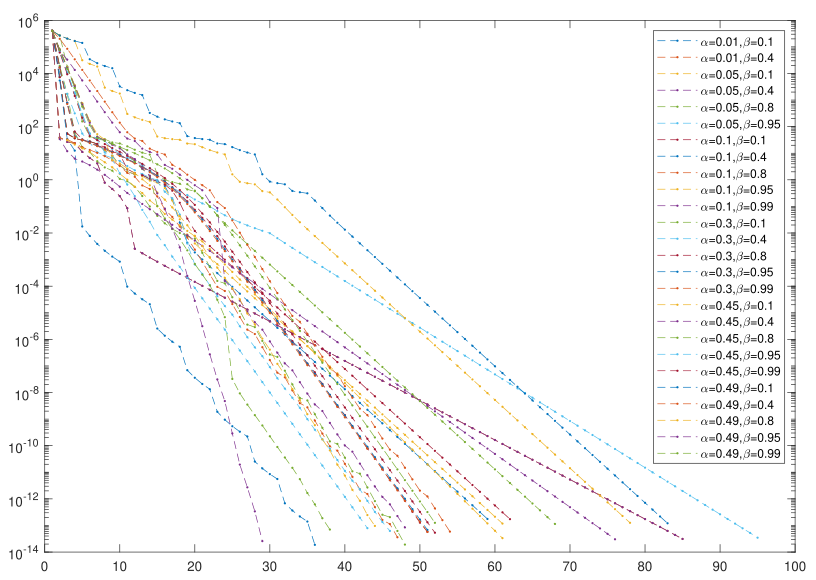
\includegraphics[scale=0.4]{Fig/group1_43.png}
        \end{minipage}
    }
    \subfigure{
        \begin{minipage}[t]{0.48\textwidth}
            \centering
            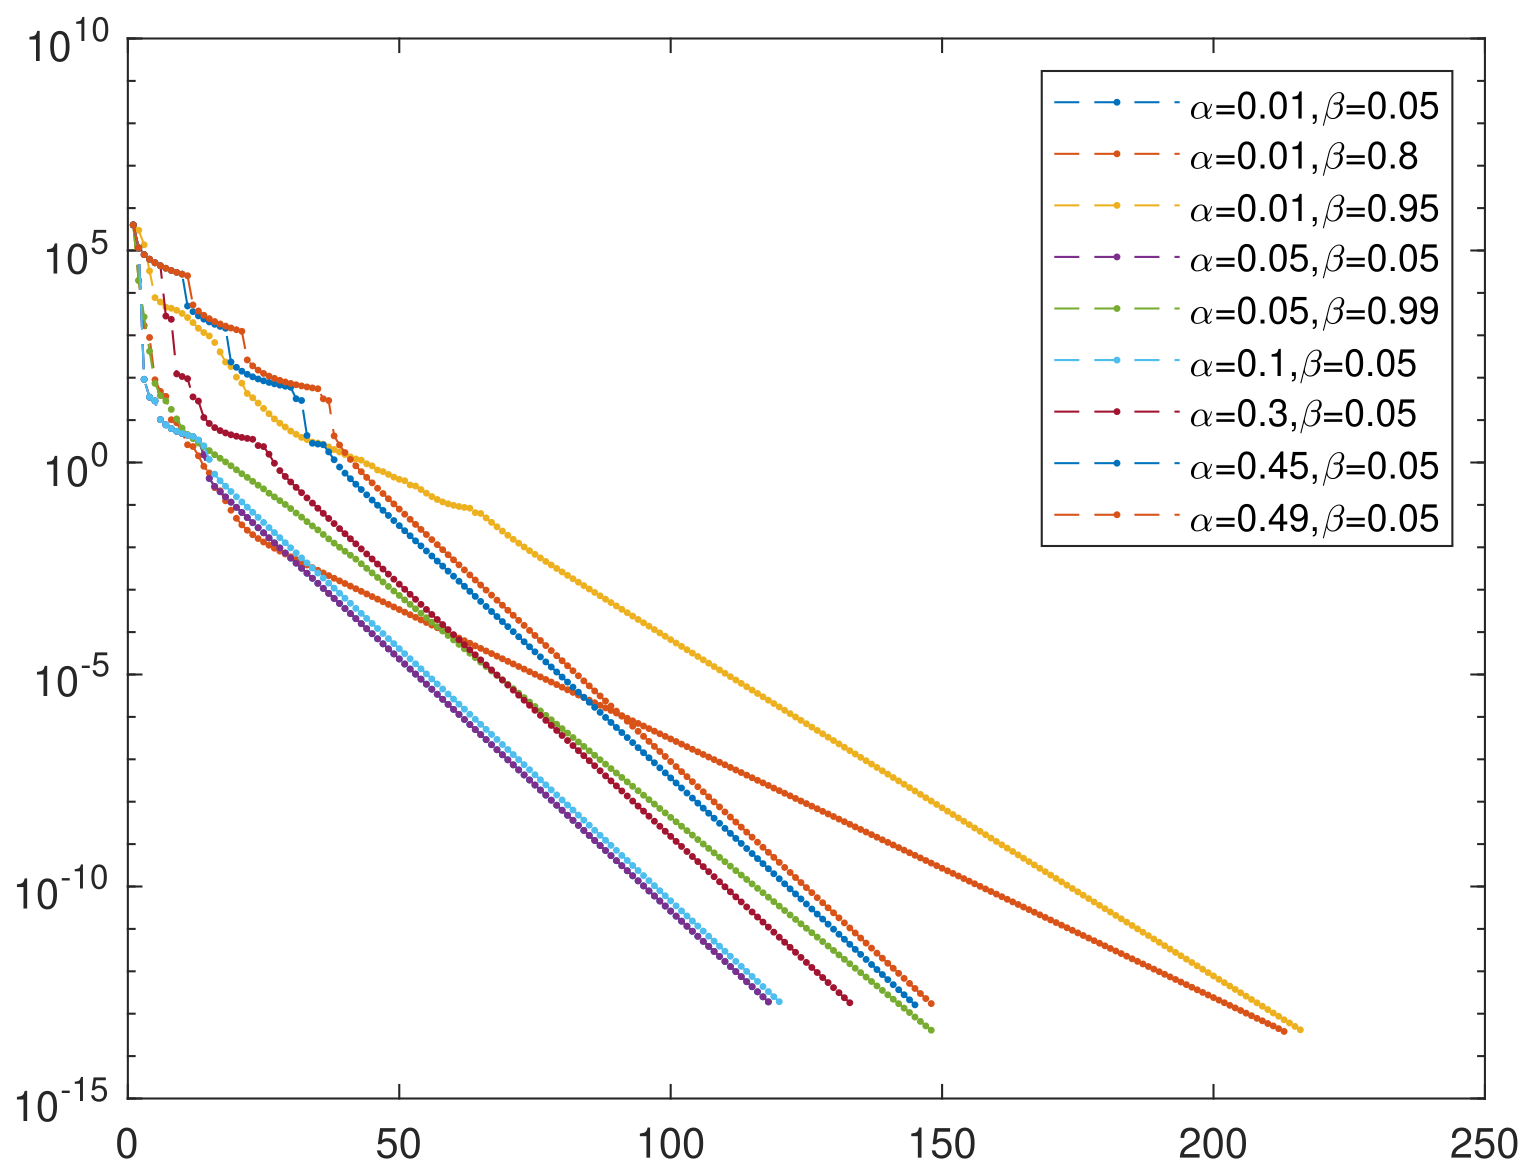
\includegraphics[scale=0.5]{Fig/group3_43.png}
        \end{minipage}
        \begin{minipage}[t]{0.48\textwidth}
            \centering
            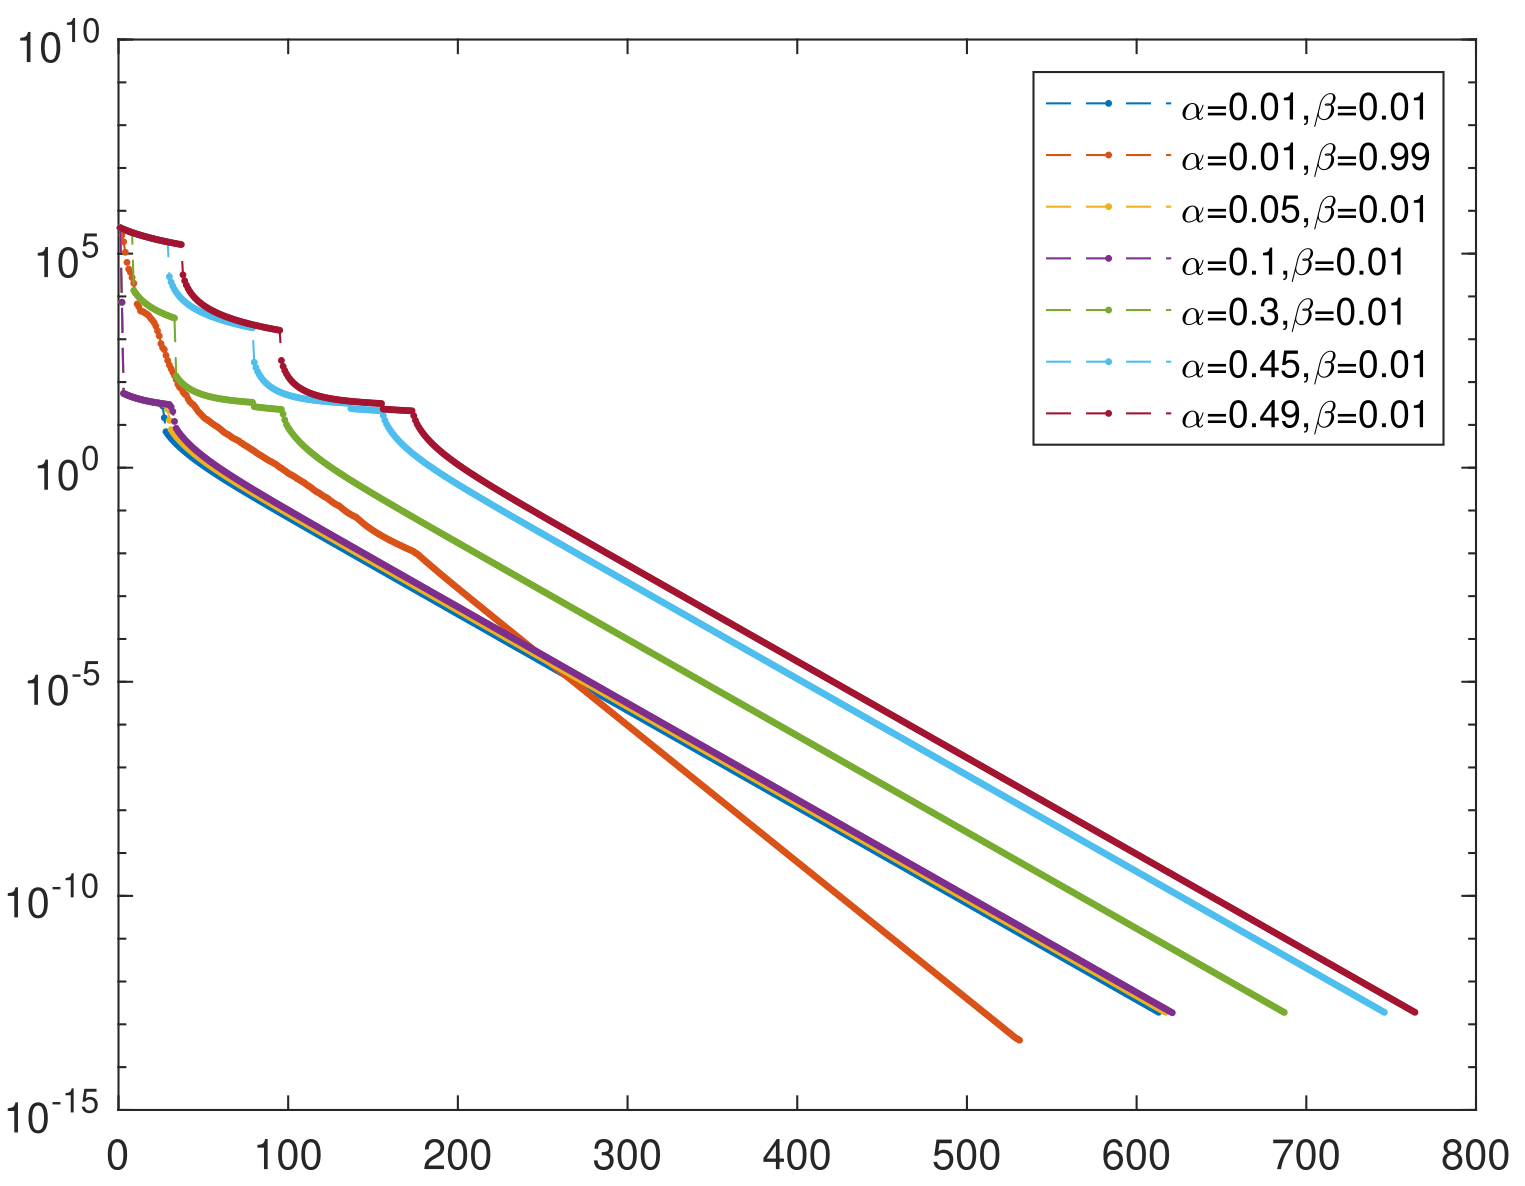
\includegraphics[scale=0.5]{Fig/group2_43.png}
        \end{minipage}
    }
    \caption{初始点$x_0=(4,3)^T$}
\end{figure}

\begin{figure}[H]
    \centering
    \subfigure{
        \begin{minipage}[t]{1\textwidth}
            \centering
            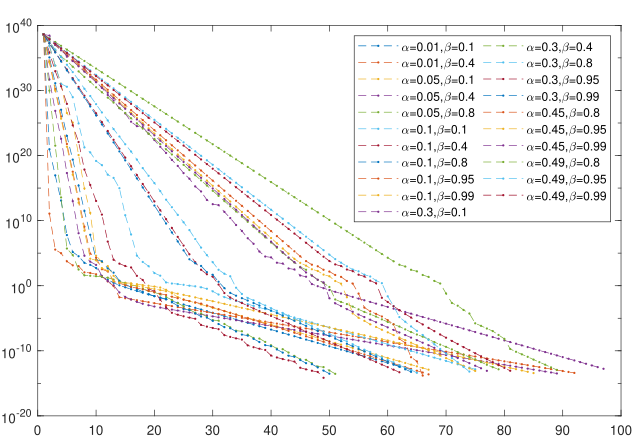
\includegraphics[scale=0.5]{Fig/group1_895.png}
        \end{minipage}
    }
    \subfigure{
        \begin{minipage}[t]{0.48\textwidth}
            \centering
            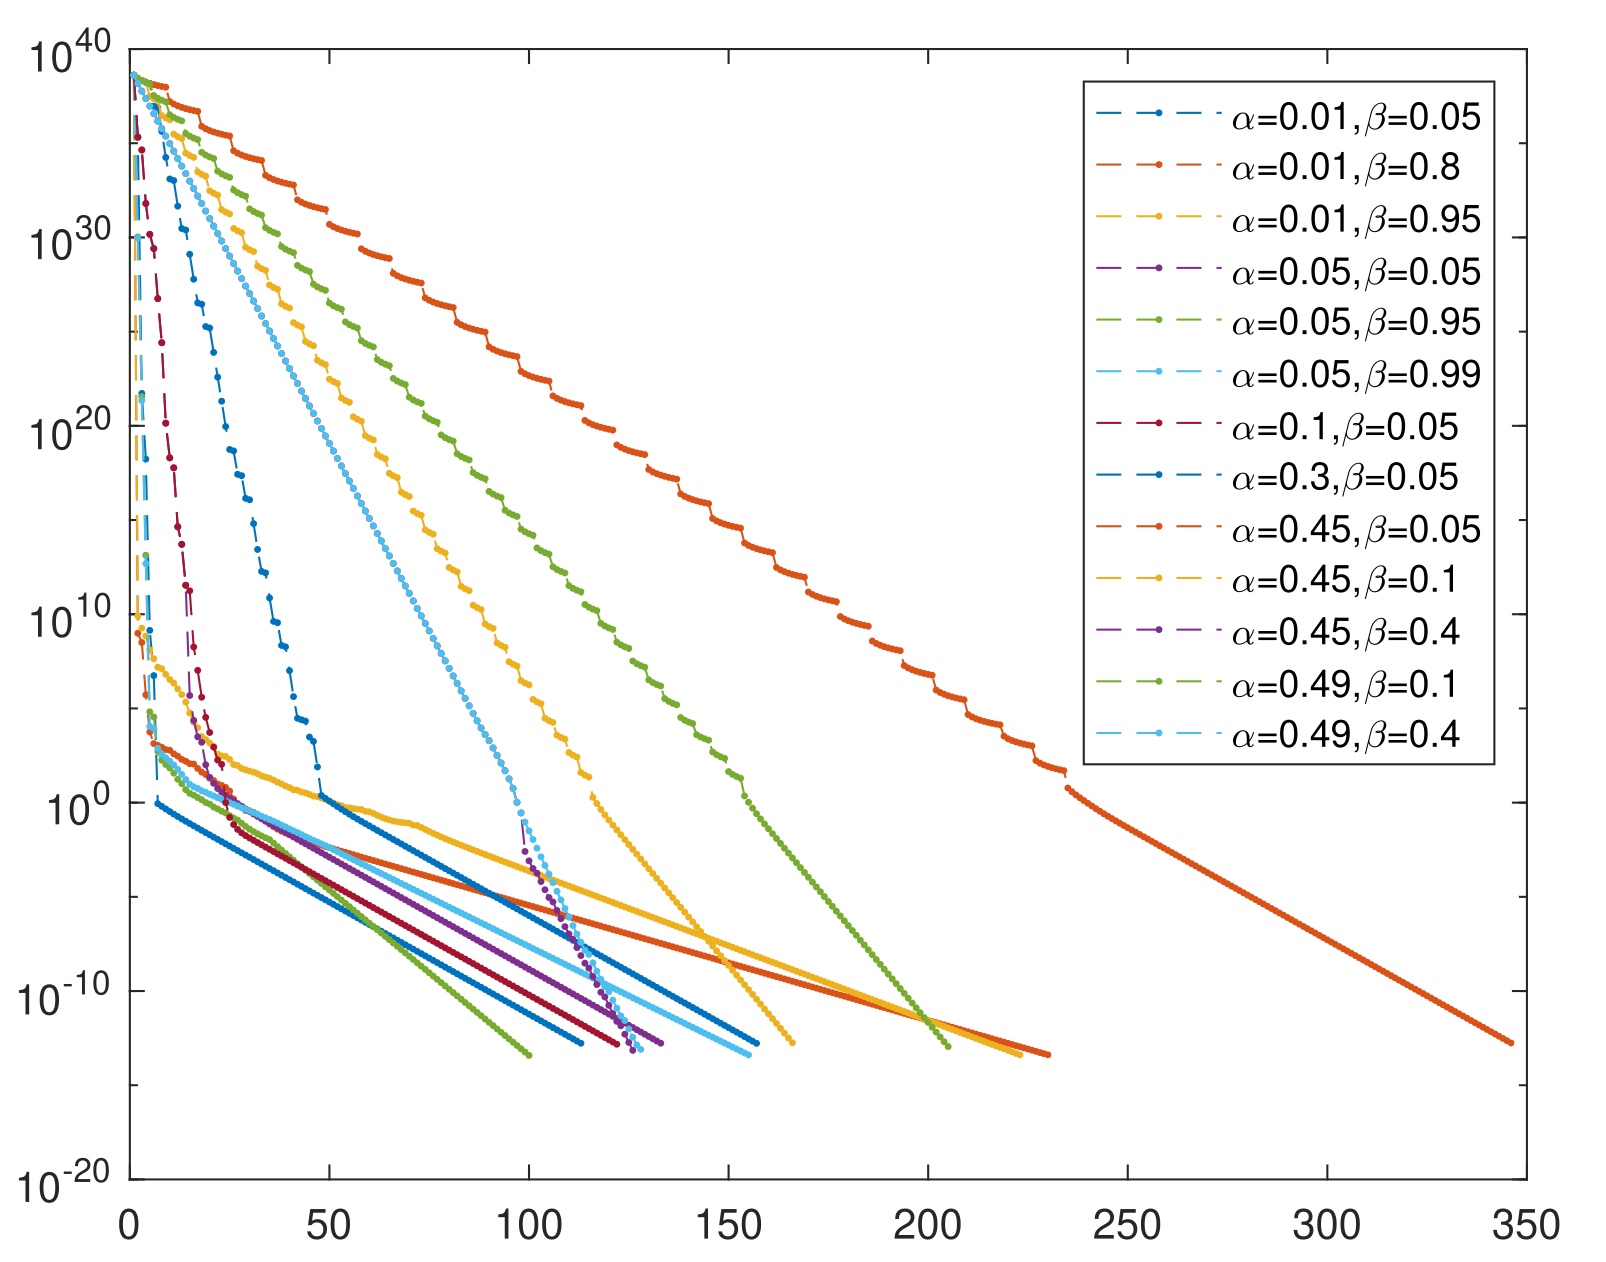
\includegraphics[width=8cm]{Fig/group3_895.png}
        \end{minipage}
        \begin{minipage}[t]{0.48\textwidth}
            \centering
            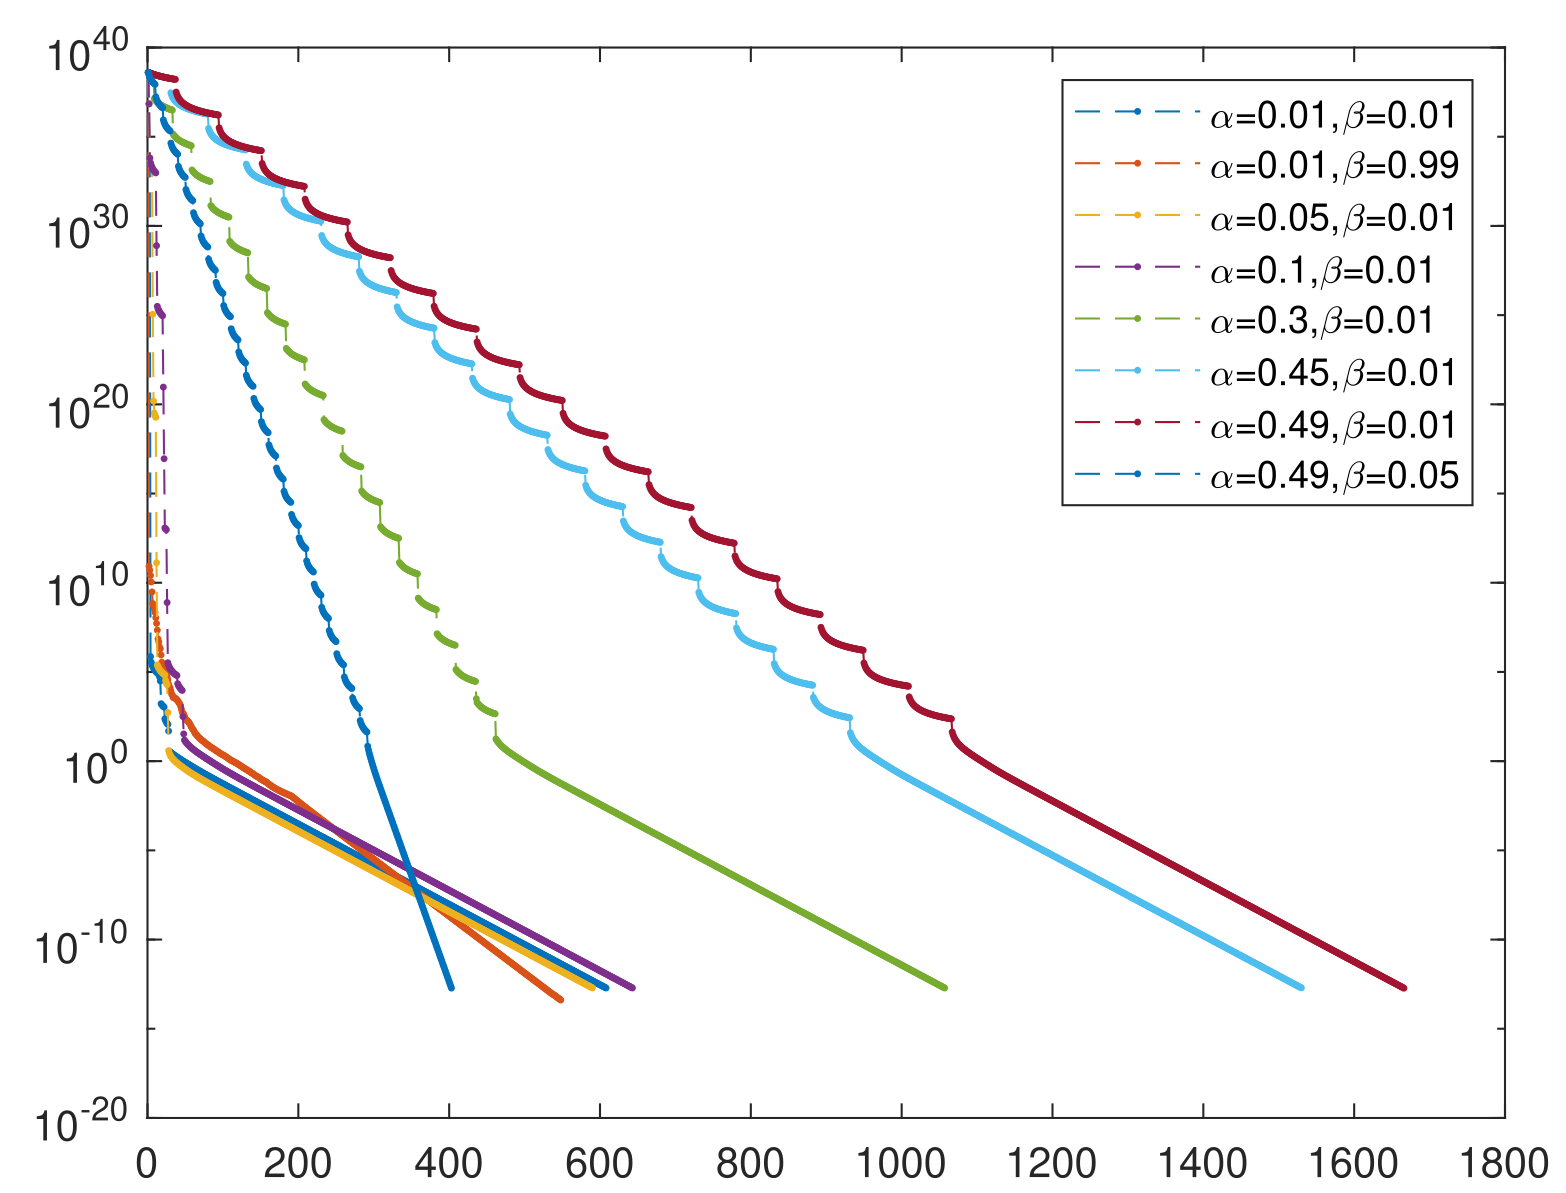
\includegraphics[width=8cm]{Fig/group2_895.png}
        \end{minipage}
    }
    \caption{初始点$x_0=(-89,5)^T$}

    \centering
    \subfigure{
        \begin{minipage}[t]{1\textwidth}
            \centering
            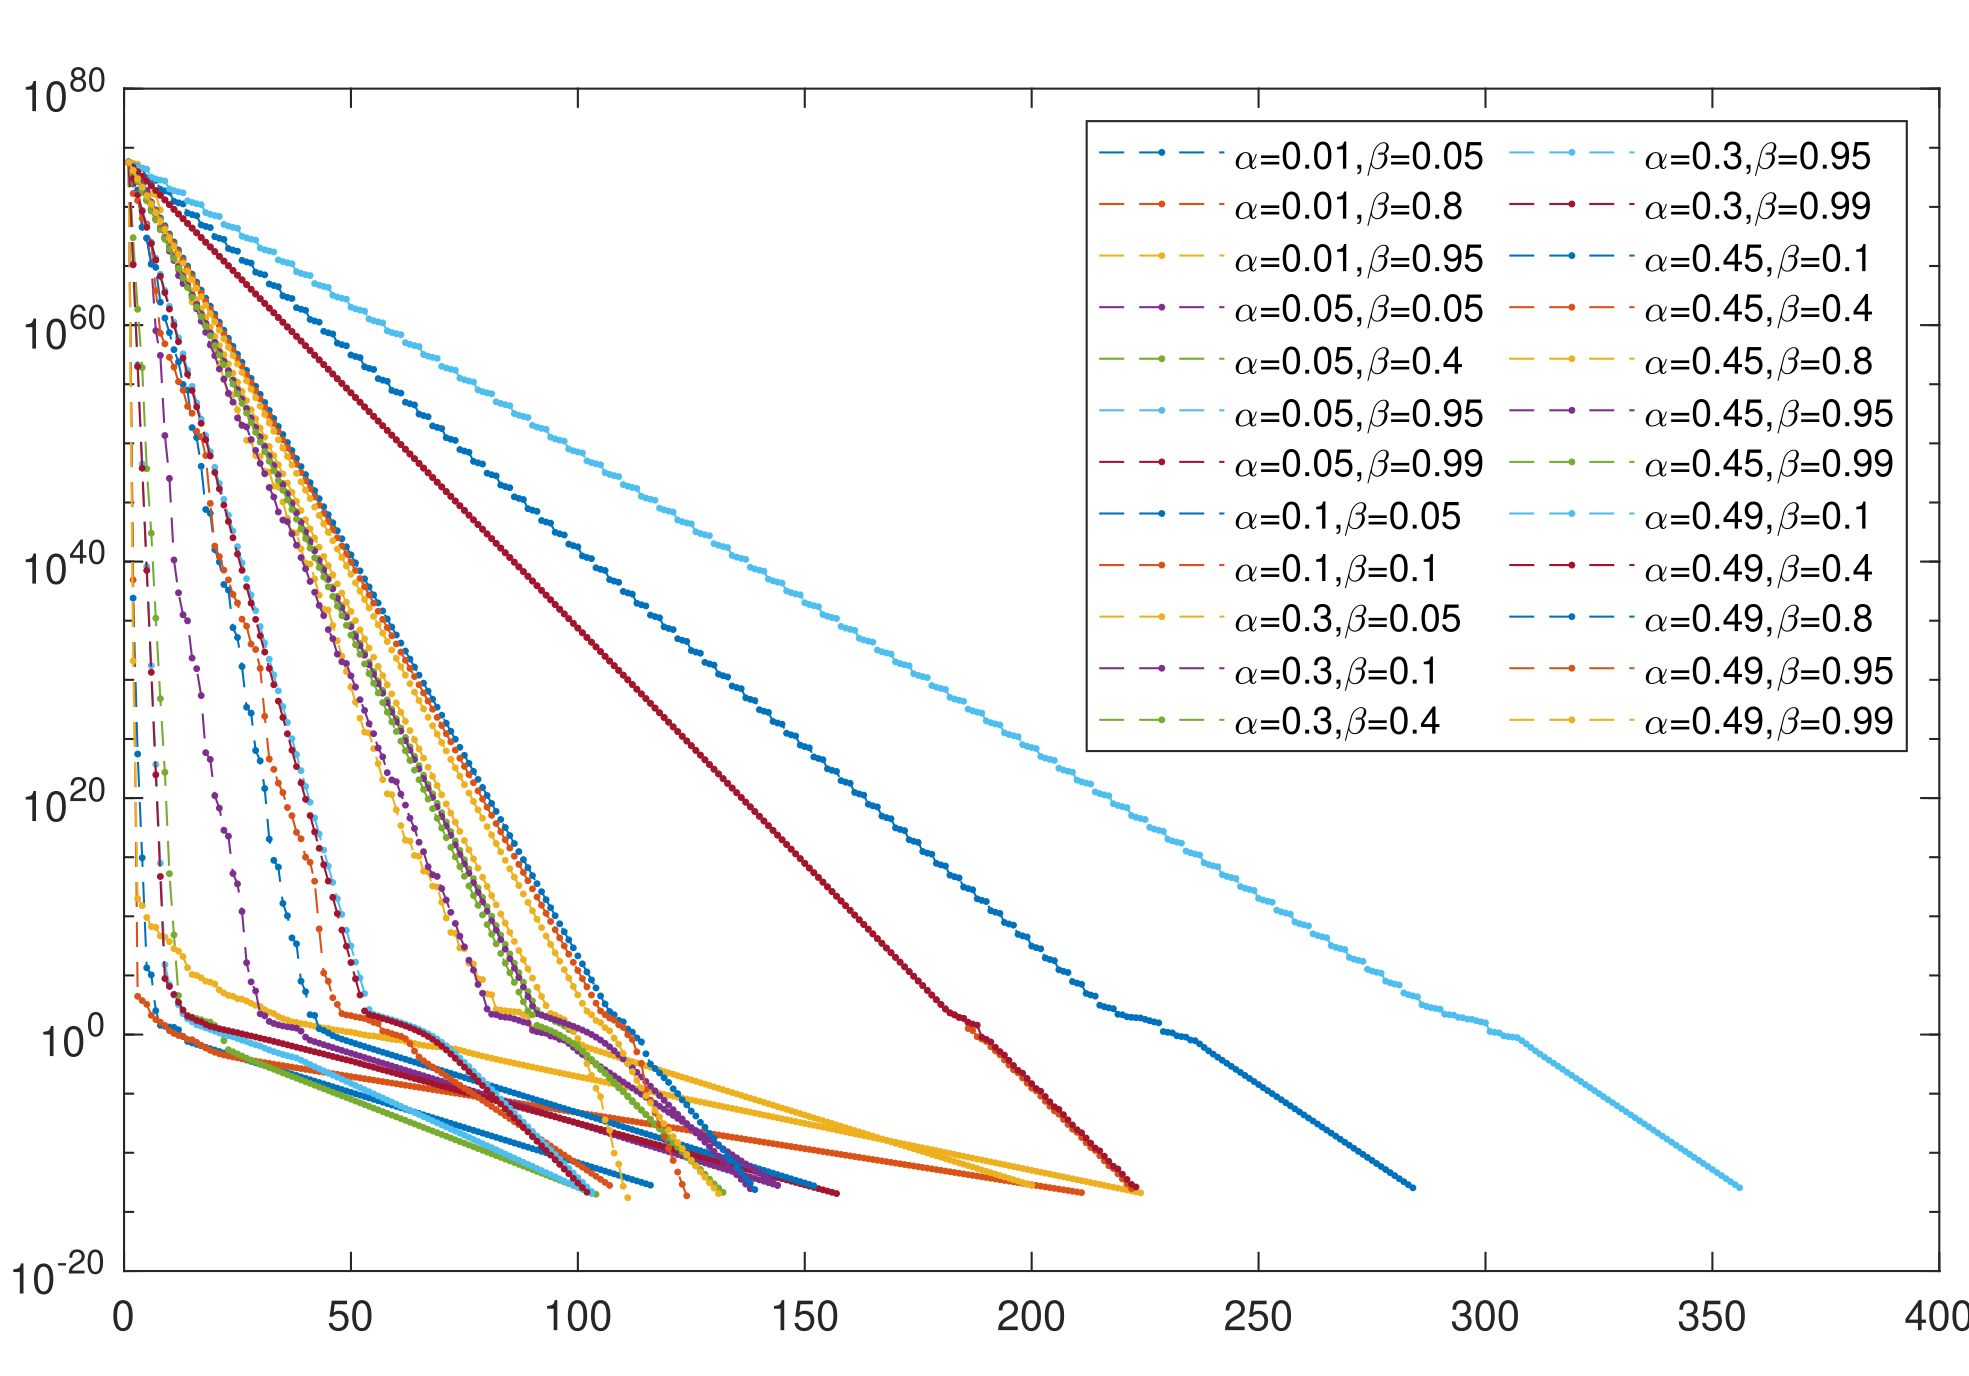
\includegraphics[scale=0.5]{Fig/group3_52.png}
        \end{minipage}
    }
    \subfigure{
        \begin{minipage}[t]{0.48\textwidth}
            \centering
            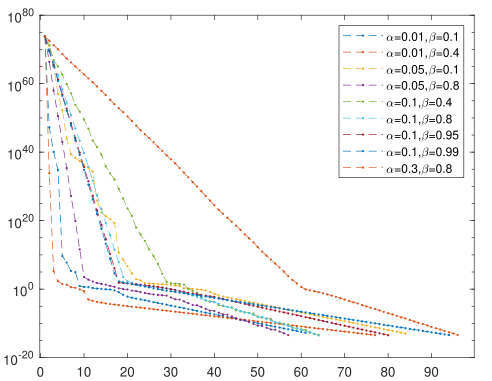
\includegraphics[width=8cm]{Fig/group1_52.png}
        \end{minipage}
        \begin{minipage}[t]{0.48\textwidth}
            \centering
            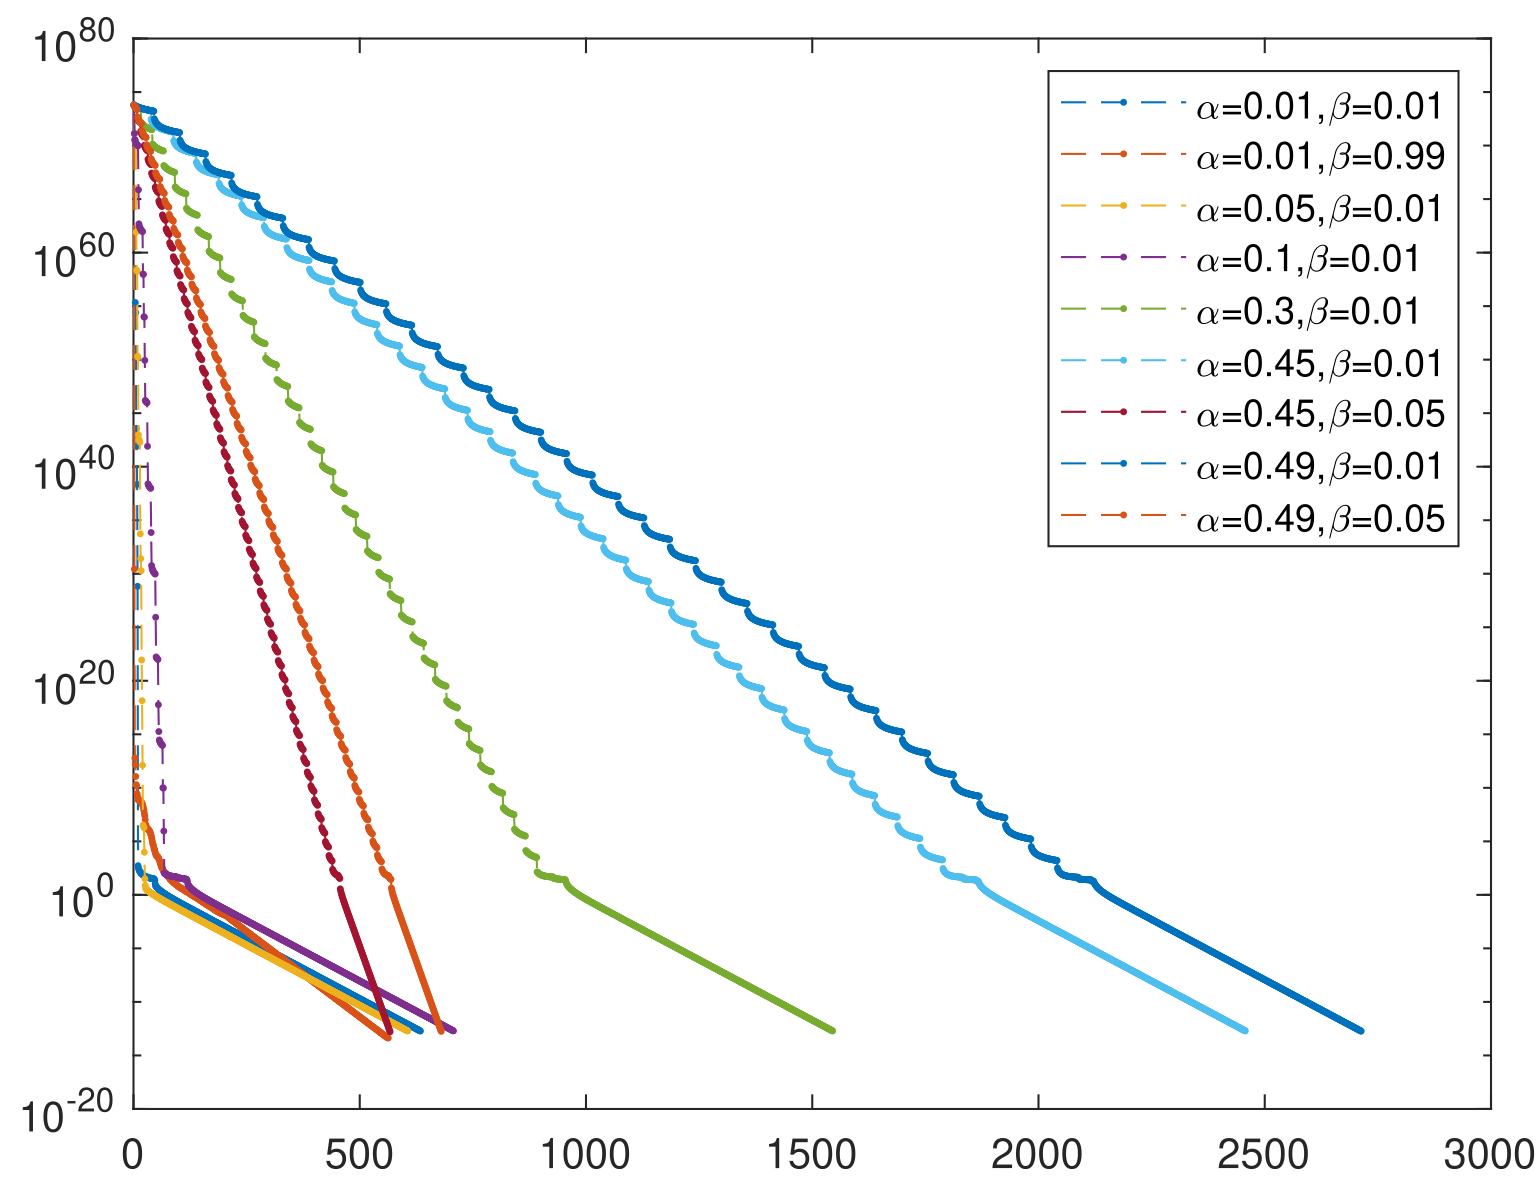
\includegraphics[width=8cm]{Fig/group2_52.png}
        \end{minipage}
    }
    \caption{初始点$x_0=(20,50)^T$}
\end{figure}

分析如下:
\begin{itemize}
    \item 在$\beta$较小时$(\beta<0.1)$,迭代次数会随着$\beta$的减小而显著增加;
    \item 在$\alpha$取值接近0或0.5,$\beta$取值接近0或1时,迭代次数也会出现较明显的增加;
    \item 在$\alpha \in \left[0.1,0,4\right],\beta \in \left[0.1,0.9\right]$的情况下,同一初始点在不同的$\alpha,\beta$取值情况下,迭代次数不会发生显著变化。
\end{itemize}


\section{P77页大作业}
\subsection{问题描述}
对于$R^2$空间的非二次规划问题$\min f(x)=e^{x_1+3x_2-0.1}+e^{x_1-3x_2-0.1}+e^{-x_1-0.1}$,分析使用$Newton$下降方法,回溯直线搜索时$\alpha=0.1,\beta=0.7$,误差随迭代次数改变的情况。

\subsection{问题思路}
由牛顿方法,下降方向$d^k_{nt}$满足:
\begin{equation*}
    d^k_{nt}=-(\nabla^2 f(x^k))^{-1} \nabla f(x^k)
\end{equation*}

牛顿减少量$\lambda^2(x^k)$满足
\begin{equation*}
    \lambda^2(x^k)={d^k_{nt}}^T \nabla^2 f(x) d^k_{nt}
\end{equation*}

由 P38页大作业所述,该问题的最优解为$\left(-\frac{1}{2}\ln 2,0\right)^T$,最优值为$p^\ast=2.559266697$,从而由牛顿下降方法生成点列$\{x^0,x^1,\dotsb,x^k \}$,即可画出$f(x^k)-p^\ast$随迭代次数改变的情况。
\\ \hspace*{\fill} \\
代码思路:
\begin{enumerate}[a)]
    \item 使用matlab符号函数(syms)求出原函数$f(x)$的梯度和$Hessian$矩阵;
    \begin{lstlisting}
    f= exp(x1+3*x2-0.1)+exp(x1-3*x2-0.1)+exp(-x1-0.1);%原函数
    grad_f=[diff(f,x1),diff(f,x2)]';%函数f的梯度
    hessian_f=hessian(f,[x1,x2]);%函数f的hessian矩阵
    \end{lstlisting}
    \item 使用matlab符号函数转匿名函数功能(matlabFunction),使其转为可代入值计算的匿名函数;
    \begin{lstlisting}
    %将上面的符号函数都转为匿名函数
    f=matlabFunction(f);
    grad_f=matlabFunction(grad_f);
    hessian_f=matlabFunction(hessian_f);
    \end{lstlisting}
    \item 外循环:判断$\frac{1}{2}\lambda^2(x^k)<10^{-6}$
    \item 内循环:通过回溯直线搜索求解$t^k$,使得$f(x^k+t^kd^k)<f(x^k)-\alpha t^k \lambda^2(x^k)$
    \begin{lstlisting}
    while (f(x_(1),x_(2)) > (f(x(1),x(2))-alpha*t*lamda_2))
        t=beta*t;
        x_=x+t*d;
    end
    \end{lstlisting}
    \item 在每次内循环结束后,记录$f(x^k)-p^\ast$,更新$x^{k+1},\lambda^2(x^k)$
    \begin{lstlisting}
    %更新参量
    x=x+t*d;
    d=-hessian_f(x(1),x(2))\grad_f(x(1),x(2));%下降方向
    lamda_2= d'*hessian_f(x(1),x(2))* d; %牛顿减少量的平方
    k=k+1;
    gap(k)=f(x(1),x(2))-p;
    \end{lstlisting}
\end{enumerate}

参数取值:
\begin{itemize}
    \item $\alpha=0.1$
    \item $\beta=0.7$
    \item 停止准则$\frac{1}{2} \lambda^2(x^k)<10^{-6}$
    \item 初始点为$x_0=(2,5)^T$
\end{itemize}


\subsection{程序运行结果}
\begin{figure}[H]
    \centering
    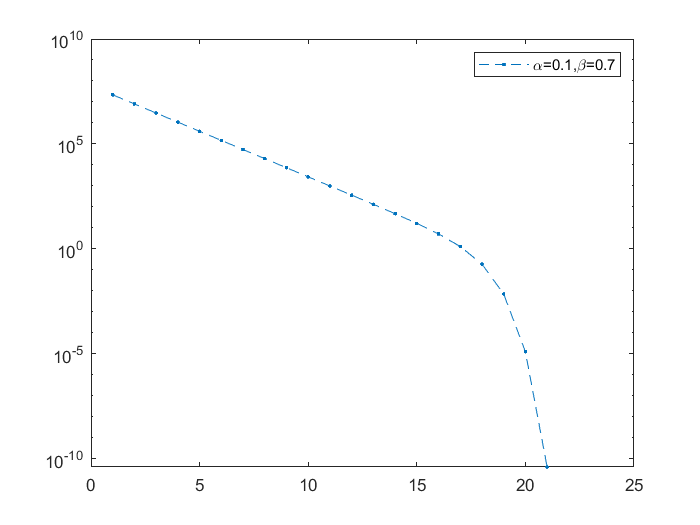
\includegraphics[width=8cm]{Fig/newton.png}
    \caption{$Newton$下降方法,$\alpha=0.1,\beta=0.7$}
\end{figure}

\end{document}